\documentclass[11pt]{article}

\usepackage[utf8]{inputenc} % character encoding - you don't need to understand this

% below are a bunch of useful packages, it doesn't cost anything to include them all so you might as well
\usepackage{amsmath}		% lets you input equations in math mode
\usepackage{graphicx}		% lets you include images
\usepackage{enumerate}		% lets you make lists
\usepackage{hyperref}		% lets you make links
\usepackage{subcaption}     % if you want to use subcaptions
\usepackage[all]{hypcap}	% makes links refer to figures and not captions
\usepackage{relsize}		% lets you use relative font sizes
\usepackage{caption}        % lets you add captions
\usepackage{array}          % lets you specify table column widths
\usepackage{siunitx}
\usepackage[margin=1in, paperwidth=8.5in, paperheight=11in]{geometry} % I'll bet you can figure this one out

% this line starts the actual document and text
\begin{document}

\title{ISIM Lab 4: A Simple Electrocardiogram (ECG/EKG)\footnote{These statements have not been evaluated by the Food and Drug Administration. This product is not intended to diagnose, treat, cure, or prevent any disease.}}
\author{Ari Porad}
\date{March 18, 2021} % leave this commented to display the current date
\maketitle % don't forget to include this line or you won't have a document header

\begin{abstract}
    A double-amplifier circuit with aggressive noise filtering was used to conduct a 1-lead Electrocardiogram (ECG or EKG). Data was analyzed to produce an EKG plot and to determine that the subject's heart rate was approximately 71 beats per minute. A commercial, FDA-cleared 1-lead EKG was used as a point of comparison and found a heart rate of 73 bpm, suggesting the system was highly accurate. A Bode plot was also computed for the system, showing that it was effective at filtering out non-heart related noise.
\end{abstract}

\section{Methodology}

\begin{figure} [!ht]
% the "!ht" will tell LaTeX to try and put the figure here, and at the top of the next page if it doesn't fit here. Getting figures to show up where you want can be a pain

	\centering  % this centers the image
	
	\includegraphics[width=1\textwidth]{circuit_diagram.jpg}
	% here I put the width as a fraction of the text width. You can also use a set number of inches, mm, pt, etc.
	% the text in the curly brackets is the name of the file. If it doesn't work, try adding the file extension, e.g. .jpg
	
	\captionsetup{margin={0.28\textwidth,0.28\textwidth}}
	% by adding margins to your caption, you can make the caption wrap with your figures rather than at the normal text width
	
	\caption{\smaller{Our measurement circuit, which consists of a double amplifier, with a total of three low-pass filters and one high-pass filter.}}
	% always caption your figures!
	
	\label{fig:circuit}
	% the label here allows me to reference this figure in text anywhere in this document. By matching the text inside the curly brackets of \label{} here and \ref{} in a paragraph, LaTeX automatically inserts the correct figure number and creates a link between the number and the referenced figure. As good practice, always use "fig:" at the beginning of figure labels
\end{figure}

For this experiment, we conducted a 1-lead electrocardiogram (EKG or ECG) on a test subject. Wikipedia defines an electrocardiogram as:\footnote{\url{https://en.wikipedia.org/w/index.php?title=Electrocardiography&oldid=1011218242}}

\begin{quote}
    [A] graph of voltage versus time of the electrical activity of the heart using electrodes placed on the skin. These electrodes detect the small electrical changes that are a consequence of cardiac muscle depolarization followed by repolarization during each cardiac cycle (heartbeat). Changes in the normal ECG pattern occur in numerous cardiac abnormalities...
\end{quote}

We conducted our EKG by applying adhesive electrodes to our participant (see Figure~\ref{fig:arm}). Leads from these electrodes were fed, in series, through two amplifiers. The left wrist was used as the voltage to be amplified, while the right wrist was used as the reference voltage. These amplifiers were used in order to drastically magnify the very very small changes in voltage measurable across human skin to a level measurable by our O-Scope. Together, they provided a total amplification of 1073 dB (as calculated via Equation~\ref{equation:gain}). Between the two amplifiers were both a high-pass and low-pass filter (with characteristic frequencies of 1.59Hz and 32.48Hz, respectively, see Equation~\ref{equation:freq}), and two more low-pass filters were placed after the final amplifier (both with characteristic frequencies of 32.48Hz, see Equation~\ref{equation:freq}). These filters served to remove as much noise as possible from our data, given that the voltage across an entire human continually fluctuates rapidly. We connected the positive and negative leads of the O-Scope to the output of the final filter and +2.5V, respectively. See Figures~\ref{fig:circuit}~\&~\ref{fig:breadboard}.

\begin{equation} \label{equation:gain}
\begin{split}
    G &= 1 + \frac{100k\Omega}{R_G} \\
    G_1 &= 1 + \frac{100k\Omega}{2k\Omega} \\
    G_2 &= 1 + \frac{100k\Omega}{4.99k\Omega} \\
    G_{total} &= G_1 * G_2 = 1073\text{ dB}
\end{split}
\end{equation}

\begin{equation} \label{equation:freq}
\begin{split}
    f &= \frac{1}{2\pi R C} \\
    f_1 &= \frac{1}{2\pi(4990\Omega)(0.000001F)} \\
    f_2 &= \frac{1}{2\pi(100000\Omega)(0.000001F)} \\
    f_3 &= \frac{1}{2\pi(499\Omega)(0.00001F)} \\
    f_4 &= \frac{1}{2\pi(4990\Omega)(0.000001F)}
\end{split}
\end{equation}

\begin{figure} [!ht]
% the "!ht" will tell LaTeX to try and put the figure here, and at the top of the next page if it doesn't fit here. Getting figures to show up where you want can be a pain

	\centering  % this centers the image
	
	\includegraphics[width=1\textwidth]{breadboard.jpg}
	% here I put the width as a fraction of the text width. You can also use a set number of inches, mm, pt, etc.
	% the text in the curly brackets is the name of the file. If it doesn't work, try adding the file extension, e.g. .jpg
	
	\captionsetup{margin={0.28\textwidth,0.28\textwidth}}
	% by adding margins to your caption, you can make the caption wrap with your figures rather than at the normal text width
	
	\caption{\smaller{Our breadboard, as used to build our circuit and measure the voltage across our test subject's heart. Longer wires can be seen running to electrodes attached to the test subject.}}
	% always caption your figures!
	
	\label{fig:breadboard}
	% the label here allows me to reference this figure in text anywhere in this document. By matching the text inside the curly brackets of \label{} here and \ref{} in a paragraph, LaTeX automatically inserts the correct figure number and creates a link between the number and the referenced figure. As good practice, always use "fig:" at the beginning of figure labels
\end{figure}
\begin{figure} [!ht]
% the "!ht" will tell LaTeX to try and put the figure here, and at the top of the next page if it doesn't fit here. Getting figures to show up where you want can be a pain

	\centering  % this centers the image
	
	\includegraphics[width=0.5\textwidth]{arm.jpg}
	% here I put the width as a fraction of the text width. You can also use a set number of inches, mm, pt, etc.
	% the text in the curly brackets is the name of the file. If it doesn't work, try adding the file extension, e.g. .jpg
	
	\captionsetup{margin={0.28\textwidth,0.28\textwidth}}
	% by adding margins to your caption, you can make the caption wrap with your figures rather than at the normal text width
	
	\caption{\smaller{An adhesive electrode applied to our test participant's arm and connected to our measurement system.}}
	% always caption your figures!
	
	\label{fig:arm}
	% the label here allows me to reference this figure in text anywhere in this document. By matching the text inside the curly brackets of \label{} here and \ref{} in a paragraph, LaTeX automatically inserts the correct figure number and creates a link between the number and the referenced figure. As good practice, always use "fig:" at the beginning of figure labels
\end{figure}

\section{Results}

\subsection{EKG Measurement}

The EKG we collected from our test subject, shown below in Figure~\ref{fig:ekg}, displays eight complete heart beats. By dividing the number of cycles in the frame by the duration of the frame, we were able to calculate that our test subject had a heart rate of 71 beats per minute.

\begin{figure} [!ht]
% the "!ht" will tell LaTeX to try and put the figure here, and at the top of the next page if it doesn't fit here. Getting figures to show up where you want can be a pain

	\centering  % this centers the image
	
	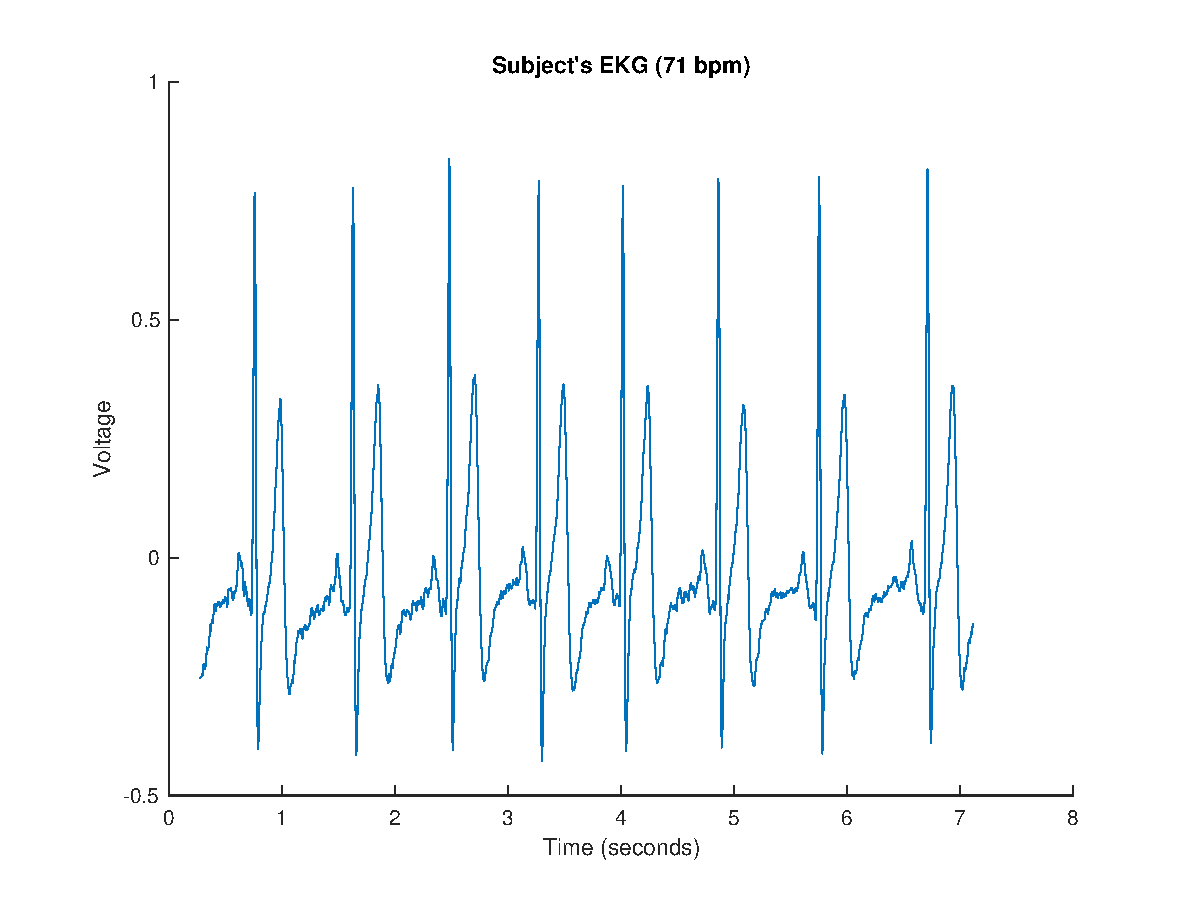
\includegraphics[width=0.75\textwidth]{ekg.eps}
	% here I put the width as a fraction of the text width. You can also use a set number of inches, mm, pt, etc.
	% the text in the curly brackets is the name of the file. If it doesn't work, try adding the file extension, e.g. .jpg
	
	\captionsetup{margin={0.28\textwidth,0.28\textwidth}}
	% by adding margins to your caption, you can make the caption wrap with your figures rather than at the normal text width
	
	\caption{\smaller{Subject's measured electrocardiogram, showing eight complete heart beats. The subject's computed heart rate was 71 beats per minute.}}
	% always caption your figures!
	
	\label{fig:ekg}
	% the label here allows me to reference this figure in text anywhere in this document. By matching the text inside the curly brackets of \label{} here and \ref{} in a paragraph, LaTeX automatically inserts the correct figure number and creates a link between the number and the referenced figure. As good practice, always use "fig:" at the beginning of figure labels
\end{figure}

\subsubsection{Comparison with Commercial EKG Device}

For comparison purposes, we also used a commercial, FDA-cleared 1-lead EKG device\footnote{Specifically, an Apple Watch Series 4's built-in EKG sensor was used: \url{https://www.theverge.com/2018/9/13/17855006/apple-watch-series-4-ekg-fda-approved-vs-cleared-meaning-safe}} to measure our subject's heart. It was not possible to conduct both measurements simultaneously because they interfered with each other, so the commercial EKG was run immediately after the conclusion of our EKG. The commercial EKG found a heart rate of 73 beats per minute, giving our system an accuracy of approximately 97\%. This high degree of accuracy gives us confidence in our approach and our system.

\subsection{Bode Plot}

\begin{figure} [!ht]
% the "!ht" will tell LaTeX to try and put the figure here, and at the top of the next page if it doesn't fit here. Getting figures to show up where you want can be a pain

	\centering  % this centers the image
	
	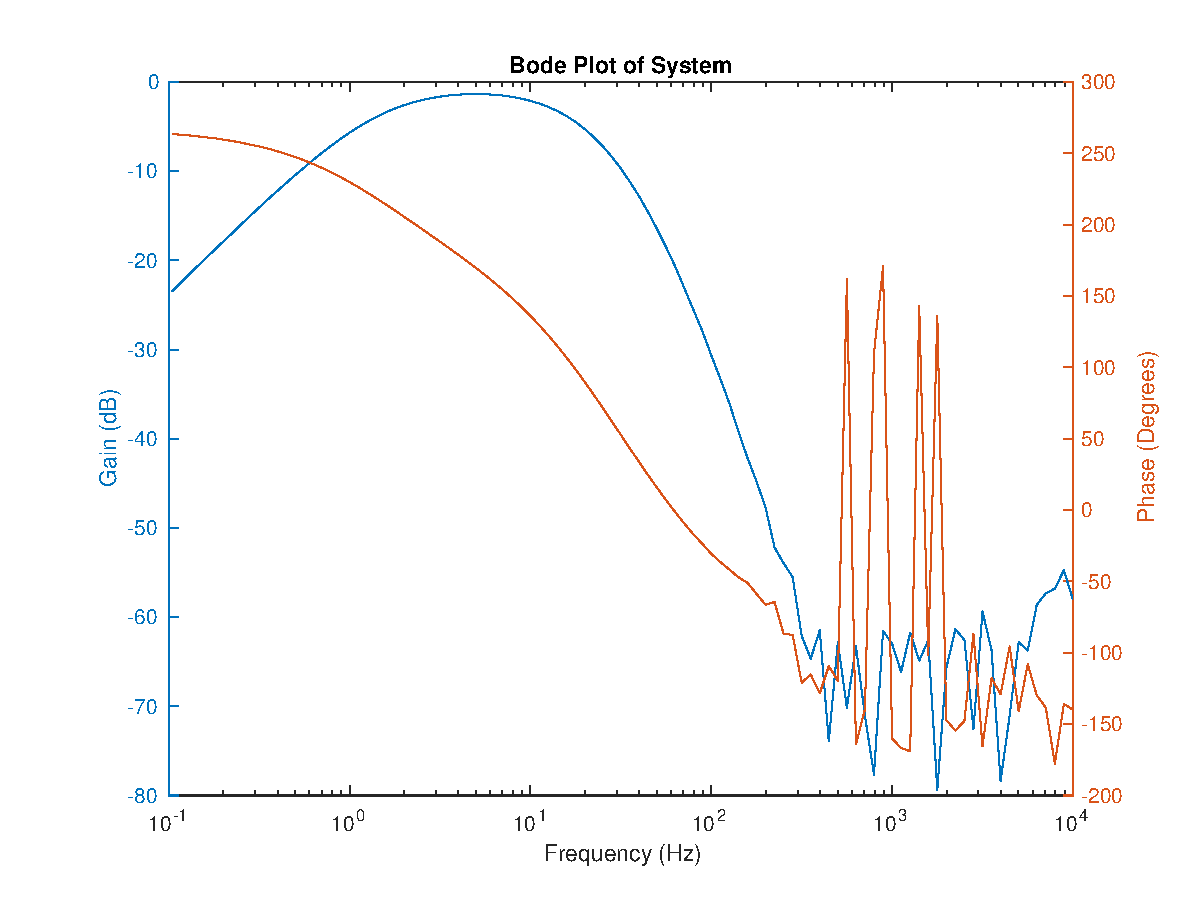
\includegraphics[width=0.75\textwidth]{bode.eps}
	% here I put the width as a fraction of the text width. You can also use a set number of inches, mm, pt, etc.
	% the text in the curly brackets is the name of the file. If it doesn't work, try adding the file extension, e.g. .jpg
	
	\captionsetup{margin={0.28\textwidth,0.28\textwidth}}
	% by adding margins to your caption, you can make the caption wrap with your figures rather than at the normal text width
	
	\caption{\smaller{Bode Plot of our system, showing gain and phase shift of our system across a range of frequencies.}}
	% always caption your figures!
	
	\label{fig:bode}
	% the label here allows me to reference this figure in text anywhere in this document. By matching the text inside the curly brackets of \label{} here and \ref{} in a paragraph, LaTeX automatically inserts the correct figure number and creates a link between the number and the referenced figure. As good practice, always use "fig:" at the beginning of figure labels
\end{figure}

From this plot, we can observe that our system has a very high gain in the 1-10 Hz range, compared to a very low gain outside that range. Given that most heart rates will fall in that 1-10Hz range, this means that the EKG signal itself will easily pass through our system while other noise will be filtered out, thereby increasing the accuracy of our measurement.


\section{Finishing Remarks}
This experiment demonstrated the ease and effectiveness of measuring an electrocardiogram with a double-amplifier circuit. Further testing is needed across a wide range of subjects to determine overall accuracy.
\end{document}